\section{Deep Learning}
\begin{multicols}{2}

As we discussed in the first week of the course, one of the key challenges in machine learning is finding the right features to use as input to a learning model for a particular problem. This is called f\emph{eature engineering} and can be part art, and part science. It can also be the single most factor in doing well on a learning task. Sometimes, in fact, more often more important than the choice of the model itself. 
We'll discuss this further in the last week of the course. 

Because of the difficulty of feature engineering, there's been a lot of research on what's called \emph{feature learning} or \emph{feature extraction} algorithms that can find good features \emph{automatically}. This brings us to deep learning. 

At a high-level, one of the advantages of deep learning is that it includes a sophisticated automatic featured learning phase as part of its supervised training. Moreover, deep learning is called deep because this feature extraction typically doesn't use just one feature learning step, but a \emph{hierarchy} of multiple feature learning layers. Each feeding into the next.

Here's one simplified example of what a deep learning architecture might look like in practice for an image recognition task. In this case, digit recognition.

\begin{center}
	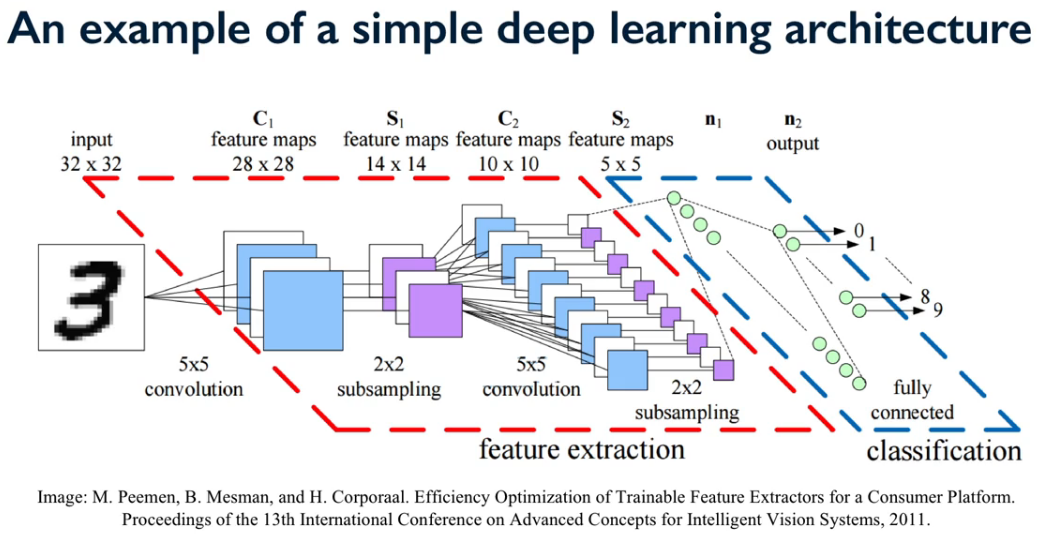
\includegraphics[width=\linewidth]{img/Deep-Learning-Architecture.png} 
\end{center} 

Recognizing a handwritten digit from zero to nine, for example. You can see the \emph{automatic feature extraction step} made up of hierarchy of feature layers. Each of which is based on a network that does \emph{convolution} which can be thought of as a filter for a specific pattern followed by a \emph{subsampling} step, also known as \emph{pooling} that can detect a translated or rotated version of that feature anywhere in the image. So that features are detected properly for the final classification step, which is implemented as a fully connected network. The subsampling step also has the effect of \emph{reducing the computational complexity} of the network. Depending on the properties of the object we want to predict, for example. If we care only about the presence of the object in the image compared to let's say, specific location, the subsampling part of the architecture may or may not be included and this is only one example of a deep learning architecture. The size, structure and other properties may look very different. Depending on the specific learning problem. 

This image from a paper by Honglak Lee and colleagues at the University of Michigan shows an illustration of multilayer feature learning for face recognition. 

Here there are three groups from left to right corresponding to first, second and third stages of feature learning. The matrix at each stage shows a set of image features with one feature per square. Each feature can be thought of as a detector or filter, that lights up when that pattern is present in the underlying image. The first layer of their deep learning architecture extracts the most primitive low-level features, such as edges and different kinds of blobs. 

The second layer creates new features from combinations of those first layer features. For faces, this might correspond to key elements that capture shapes of higher level features like noses or eyes. 

The third layer in turn, creates new features from combinations of the second layer of features. Forming still higher level features that capture typical face types and facial expressions. Finally, all of these features are used as input to the final supervised learning step, namely the face classifier. Here are the feature layers that result from training on different types of objects, cars, elephants, chairs and a mixture of objects. 

These kinds of complex features can't be learned from a small number of layers. Advances in both algorithms and computing power allow current deep learning systems to train architectures that could have dozens of layers of nonlinear, hierarchical features. It turns out that the human brain does something quite related to this when processing visual information. There are specific neurocircuits that first do low-level feature extraction, such as edge detection and finding the frequency of repeated patterns which are then used to compute more sophisticated features to help estimate things like simple shapes and their orientation or whether a shape is in the foreground or background. Followed by further layers of higher level visual processing that support more complex tasks, such as face recognition and interpreting the motion of multiple moving objects.

\subsection{Pros and Cons}

On the \textbf{positive} side, deep learning systems have achieved impressive gains and have achieved state-of-the-art \emph{performance} on many difficult tasks. 

Deep learning's automatic feature extraction mechanisms also \emph{reduce the need for human guesswork} in finding good features. 

Finally, with current software, deep learning architectures are quite \emph{flexible}. It could be adapted for different tasks and domains. 

On the \textbf{negative} side, however, deep learning can \emph{require very large training sets and computing power}. I'm not going to limit its practicality in some scenarios. 

The \emph{complexity of implementation} could be considered as one of the negatives of deep learning and this is the reason that a number of sophisticated high-level software packages have been developed to assist in the development of deep learning architectures. 

Also, despite the faces example we saw earlier which gave clear easy to interpret features in most cases, often the features and weights of typical deep learning systems are \emph{not easy to interpret}. That is, it's not clear why or what features led a deep learning system to make a particular prediction. 

Well, scikit-learn with the \texttt{MLPСlassifier} and \texttt{MLPКegressor} classes provides a useful environment to learn about and apply simple neural networks. If you're interested in getting a deep understanding of deep learning and the software tools required to use it, we've provided some links to additional resources. 

In particular, software packages usable with Python include \texttt{Keras} and \texttt{Lasagne} which in turn use libraries that include \texttt{TensorFlow} and \texttt{Theano}.

Deep learning typically requires not only significant volumes of data for training, but also \emph{significant computation}. Turns out that the processor inside video cards called \textbf{GPUs} are high-performance graphical processing units are well-suited to large scale, highly paralyzed high-performance computing. Because they can do high key underlying like matrix multiplication very quickly. This is because they are designed to process large volumes of data from memory as you might do for streaming video, for example, and they have many high speed registers that can operate in parallel on this data. 

Unlike \texttt{scikit-learn} which \emph{cannot} currently exploit GPUs, these deep learning libraries could make full use of GPU clusters for large scale learning of deep learning architectures. 

\end{multicols}